\documentclass[oneside]{book}\usepackage[]{graphicx}\usepackage[]{color}
% maxwidth is the original width if it is less than linewidth
% otherwise use linewidth (to make sure the graphics do not exceed the margin)
\makeatletter
\def\maxwidth{ %
  \ifdim\Gin@nat@width>\linewidth
    \linewidth
  \else
    \Gin@nat@width
  \fi
}
\makeatother

\definecolor{fgcolor}{rgb}{0.345, 0.345, 0.345}
\newcommand{\hlnum}[1]{\textcolor[rgb]{0.686,0.059,0.569}{#1}}%
\newcommand{\hlstr}[1]{\textcolor[rgb]{0.192,0.494,0.8}{#1}}%
\newcommand{\hlcom}[1]{\textcolor[rgb]{0.678,0.584,0.686}{\textit{#1}}}%
\newcommand{\hlopt}[1]{\textcolor[rgb]{0,0,0}{#1}}%
\newcommand{\hlstd}[1]{\textcolor[rgb]{0.345,0.345,0.345}{#1}}%
\newcommand{\hlkwa}[1]{\textcolor[rgb]{0.161,0.373,0.58}{\textbf{#1}}}%
\newcommand{\hlkwb}[1]{\textcolor[rgb]{0.69,0.353,0.396}{#1}}%
\newcommand{\hlkwc}[1]{\textcolor[rgb]{0.333,0.667,0.333}{#1}}%
\newcommand{\hlkwd}[1]{\textcolor[rgb]{0.737,0.353,0.396}{\textbf{#1}}}%
\let\hlipl\hlkwb

\usepackage{framed}
\makeatletter
\newenvironment{kframe}{%
 \def\at@end@of@kframe{}%
 \ifinner\ifhmode%
  \def\at@end@of@kframe{\end{minipage}}%
  \begin{minipage}{\columnwidth}%
 \fi\fi%
 \def\FrameCommand##1{\hskip\@totalleftmargin \hskip-\fboxsep
 \colorbox{shadecolor}{##1}\hskip-\fboxsep
     % There is no \\@totalrightmargin, so:
     \hskip-\linewidth \hskip-\@totalleftmargin \hskip\columnwidth}%
 \MakeFramed {\advance\hsize-\width
   \@totalleftmargin\z@ \linewidth\hsize
   \@setminipage}}%
 {\par\unskip\endMakeFramed%
 \at@end@of@kframe}
\makeatother

\definecolor{shadecolor}{rgb}{.97, .97, .97}
\definecolor{messagecolor}{rgb}{0, 0, 0}
\definecolor{warningcolor}{rgb}{1, 0, 1}
\definecolor{errorcolor}{rgb}{1, 0, 0}
\newenvironment{knitrout}{}{} % an empty environment to be redefined in TeX

\usepackage{alltt}
\usepackage[svgnames]{xcolor}
\usepackage[british]{babel}
\usepackage[protrusion,expansion,babel,final]{microtype}
\usepackage[margin=1in]{geometry}
\usepackage[pdfversion=1.7]{hyperref}
\usepackage[shortlabels]{enumitem}
\usepackage{graphicx}
\usepackage{mathtools}
\usepackage{cleveref}
\usepackage{booktabs}
\usepackage{nicematrix}
\usepackage{derivative}
\usepackage{etoolbox}
\usepackage{siunitx}
\usepackage{lmodern}
\usepackage[T1]{fontenc}
\usepackage[scaled=.98]{XCharter}
\usepackage[scaled=1.04,varqu,varl]{inconsolata}% inconsolata typewriter
\usepackage{amssymb}
\makeatletter
\@namedef{T1/zi4/m/it}{<->ssub*lmr/m/it}
\makeatother

\usepackage{bm}
\usepackage{tikz}
\usepackage{float}

% Functions
\providecommand\given{} % just to make sure it exists
\DeclarePairedDelimiterXPP{\E}[1]{\operatorname{\mathbb{E}}}[]{}{%
    \renewcommand\given{\nonscript\:\delimsize\vert\nonscript\:\mathopen{}}%
    \ifblank{#1}{\:\cdot\:}%
    #1}%
\DeclarePairedDelimiterXPP{\V}[1]{\operatorname{\textsf{V}}}(){}{%
    \renewcommand\given{\nonscript\:\delimsize\vert\nonscript\:\mathopen{}}%
    \ifblank{#1}{\:\cdot\:}%
    #1}%
\DeclarePairedDelimiterXPP{\Var}[1]{\operatorname{\textsf{Var}}}(){}{%
    \renewcommand\given{\nonscript\:\delimsize\vert\nonscript\:\mathopen{}}%
    \ifblank{#1}{\:\cdot\:}%
    #1}%
\DeclarePairedDelimiterXPP{\Cov}[1]{\operatorname{\textsf{Cov}}}(){}{%
    \renewcommand\given{\nonscript\:\delimsize\vert\nonscript\:\mathopen{}}%
    \ifblank{#1}{\:\cdot\:}%
    #1}%
\DeclarePairedDelimiterXPP{\Corr}[1]{\operatorname{\textsf{Corr}}}(){}{%
    \renewcommand\given{\nonscript\:\delimsize\vert\nonscript\:\mathopen{}}%
    \ifblank{#1}{\:\cdot\:}%
    #1}%
\DeclarePairedDelimiterXPP{\Covadj}[1]{\operatorname{\textsf{Cov}_{\text{adj}}}}(){}{%
    \renewcommand\given{\nonscript\:\delimsize\vert\nonscript\:\mathopen{}}%
    \ifblank{#1}{\:\cdot\:}%
    #1}%
\DeclarePairedDelimiterXPP\Prob[1]{\operatorname{\mathbb{P}}}(){}{%
    \renewcommand\given{\nonscript\:\delimsize\vert\nonscript\:\mathopen{}}%
    \ifblank{#1}{\:\cdot\:}%
    #1}%
\DeclarePairedDelimiterXPP\Ind[1]{\operatorname{\mathbb{I}}}\{\}{}{%
    \renewcommand\given{\nonscript\:\delimsize\vert\nonscript\:\mathopen{}}%
    \ifblank{#1}{\:\cdot\:}%
    #1}%
\DeclarePairedDelimiterXPP{\se}[1]{\operatorname{\textsf{se}}}(){}{%
    \ifblank{#1}{\:\cdot\:}%
    #1}%
\DeclarePairedDelimiterXPP{\seadj}[1]{\operatorname{\textsf{se}_{\text{adj}}}}(){}{%
    \renewcommand\given{\nonscript\:\delimsize\vert\nonscript\:\mathopen{}}%
    \ifblank{#1}{\:\cdot\:}%
    #1}%
\DeclarePairedDelimiterXPP{\estseadj}[1]{\operatorname{\widehat{\textsf{se}}_{\text{adj}}}}(){}{%
    \renewcommand\given{\nonscript\:\delimsize\vert\nonscript\:\mathopen{}}%
    \ifblank{#1}{\:\cdot\:}%
    #1}%
\DeclarePairedDelimiterXPP{\estse}[1]{\widehat{\operatorname{\textsf{se}}}}(){}{%
    \ifblank{#1}{\:\cdot\:}%
    #1}%
\DeclarePairedDelimiterXPP{\estV}[1]{\widehat{\operatorname{\textsf{V}}}}(){}{
    \renewcommand\given{\nonscript\:\delimsize\vert\nonscript\:\mathopen{}}%
    \ifblank{#1}{\:\cdot\:}%
    #1}%
\DeclarePairedDelimiterXPP{\estVar}[1]{\widehat{\operatorname{\textsf{Var}}}}(){}{
    \renewcommand\given{\nonscript\:\delimsize\vert\nonscript\:\mathopen{}}%
    \ifblank{#1}{\:\cdot\:}%
    #1}%
\let\exp\relax%
\let\log\relax%
\let\ln\relax%
\DeclarePairedDelimiterXPP{\exp}[1]{\operatorname{\textsf{exp}}}\{\}{}{#1}%
\DeclarePairedDelimiterXPP{\log}[1]{\operatorname{\textsf{log}}}(){}{#1}%
\DeclarePairedDelimiterXPP{\ln}[1]{\operatorname{\textsf{ln}}}(){}{#1}%
\DeclarePairedDelimiterXPP{\diag}[1]{\operatorname{\textsf{diag}}}(){}{#1}%
\DeclarePairedDelimiterXPP{\sign}[1]{\operatorname{\textsf{sign}}}(){}{#1}%

\DeclarePairedDelimiterXPP{\expit}[1]{\operatorname{\textsf{expit}}}(){}{#1}%
\DeclarePairedDelimiterXPP{\logit}[1]{\operatorname{\textsf{logit}}}(){}{#1}%
\newcommand{\HN}{\textsl{H}_{\textsl{0}}}%
\newcommand{\HA}{\textsl{H}_{\textsl{A}}}%

% Distributions
\DeclarePairedDelimiterXPP{\N}[1]{\mathcal{N}}(){}{#1}%
\DeclarePairedDelimiterXPP{\POI}[1]{\text{POI}}(){}{#1}%
\DeclarePairedDelimiterXPP{\BIN}[1]{\text{BIN}}(){}{#1}%
\DeclarePairedDelimiterXPP{\BERN}[1]{\text{BERN}}(){}{#1}%
\DeclarePairedDelimiterXPP{\MVN}[1]{\text{MVN}}(){}{#1}%
\DeclarePairedDelimiterXPP{\NB}[1]{\text{NB}}(){}{#1}%
\DeclarePairedDelimiterXPP{\GAM}[1]{\text{GAM}}(){}{#1}%
\DeclarePairedDelimiterXPP{\BetaDist}[1]{\text{Beta}}(){}{#1}%

\newcommand{\iid}{\overset{\text{iid}}{\sim}}%
\newcommand{\ind}{\overset{\text{ind}}{\sim}}%
\newcommand{\OR}{\text{OR}}%
\newcommand{\RR}{\text{RR}}%
\newcommand{\cOR}{\text{cOR}}%

\DeclarePairedDelimiter\abs{\lvert}{\rvert}
% can be useful to refer to this outside \Set
\newcommand\SetSymbol[1][]{%
    \nonscript\:#1\vert{}
    \allowbreak\nonscript\:
    \mathopen{}}
\DeclarePairedDelimiterX\Set[1]\{\}{%
    \renewcommand\given{:}
    #1
}
\DeclareMathOperator*{\argmax}{arg\,max}
\DeclareMathOperator*{\argmin}{arg\,min}
\DeclareMathOperator*{\arginf}{arg\,inf}
\DeclareMathOperator*{\argsup}{arg\,sup}

\providecommand{\RandomVector}[1]{\bm{#1}}% general vectors in bold italic
\providecommand{\Vector}[1]{\bm{#1}}% general vectors in bold italic
\providecommand{\Matrix}[1]{\bm{#1}}
\providecommand{\MatrixCal}[1]{\bm{\mathcal{#1}}}
\providecommand{\Field}[1]{\bm{#1}}

\usepackage{stackengine}
\usepackage[british]{isodate}
\newcommand{\makeheading}[2]%
{%
\begin{center}%
    \makebox[\linewidth]{\raisebox{-.5ex}[0cm][0cm]{\stackanchor{\textcolor{Gray}{\textsc{#1}}}{\scriptsize\itshape\printyearoff#2}\;}\color{Crimson!50}\hrulefill}%
\end{center}%
}%

\usepackage[breakable]{tcolorbox}
\tcbset{
    regular/.style={
        boxrule=0pt,
        breakable,
        sharp corners
    }
}

\newtcolorbox{Example}[1]{regular,colframe=Green!20!white,colback=Green!10!white,coltitle=Green,title={#1}}%
\newtcolorbox{Regular}[1]{regular,colframe=Navy!15!white,colback=Navy!5!white,coltitle=Navy,title={#1}}%
\newtcolorbox{Result}[1]{regular,colframe=Red!15!white,colback=Red!5!white,coltitle=Red,title={#1}}%

\hypersetup{colorlinks=true,%
linkcolor=[rgb]{0,0.5,1},%
pdftitle={Generalized Linear Models and their Applications (STAT 431/STAT 831)},%
pdfauthor={Cameron Roopnarine, Leilei Zeng},%
pdfsubject={Statistics},%
pdfkeywords={University of Waterloo, Fall 2021 (1219)}}%

\title{%
\LARGE Generalized Linear Models and their Applications\\%
\large STAT 431/STAT 831\thanks{STAT 431 $ \equiv $ STAT 831}\\%
\normalsize Fall 2021 (1219)\thanks{Online Course}}%
\author{Cameron Roopnarine\thanks{\LaTeX{}er}\and Leilei Zeng\thanks{Instructor}}%
\date{\today}%
\usepackage{pgfplots}
\pgfplotsset{compat=1.18}
\usetikzlibrary{petri,decorations.pathreplacing,calc}
\usepackage{framed}
\IfFileExists{upquote.sty}{\usepackage{upquote}}{}
\begin{document}

\setcounter{chapter}{5}
\chapter{Gaussian Response Models}
\section{Gaussian Response Models Part I}
\subsection{Introduction}
\begin{Example}{Example: STAT 230 and 231 Final Grades}
    \begin{center}
        \begin{NiceTabular}{|c|c|c|}
            \toprule
            \text{No.} & \text{S230} & \text{S231} \\
            \midrule
            1          & 76          & 76          \\
            2          & 77          & 79          \\
            3          & 57          & 54          \\
            4          & 75          & 64          \\
            5          & 74          & 64          \\
            6          & 60          & 60          \\
            7          & 81          & 85          \\
            8          & 86          & 82          \\
            9          & 96          & 88          \\
            10         & 79          & 72          \\
            \bottomrule
        \end{NiceTabular}\hfill
        \begin{NiceTabular}{|c|c|c|}
            \toprule
            \text{No.} & \text{S230} & \text{S231} \\
            \midrule
            11         & 87          & 76          \\
            12         & 71          & 50          \\
            13         & 63          & 75          \\
            14         & 77          & 72          \\
            15         & 96          & 84          \\
            16         & 65          & 69          \\
            17         & 71          & 43          \\
            18         & 66          & 60          \\
            19         & 90          & 96          \\
            20         & 50          & 50          \\
            \bottomrule
        \end{NiceTabular}\hfill
        \begin{NiceTabular}{|c|c|c|}
            \toprule
            \text{No.} & \text{S230} & \text{S231} \\
            \midrule
            21         & 98          & 83          \\
            22         & 80          & 88          \\
            23         & 67          & 52          \\
            24         & 78          & 75          \\
            25         & 100         & 99          \\
            26         & 94          & 94          \\
            27         & 83          & 83          \\
            28         & 51          & 37          \\
            29         & 77          & 90          \\
            30         & 77          & 67          \\
            \bottomrule
        \end{NiceTabular}
    \end{center}
    \begin{framed}
        \begin{itemize}
            \item Why might we be interested in collecting data such as these?
            \item What might be a reasonable choice for the target and study population?
            \item What are the variates? What type are they?
            \item What is the explanatory variate? What is the response variate?
            \item How do we summarize these data numerically and graphically?
            \item What model could we use to analyse these data?
        \end{itemize}
    \end{framed}
\end{Example}
\subsection{Sample Correlation}
Recall that the sample correlation is a numerical measure of the linear relationship between two variates.
It is defined as
\[ r =\frac{S_{x y}}{\sqrt{S_{x x} S_{y y}}}, \]
where
\begin{align*}
    S_{x x} & =\sum_{i=1}^{n}(x_{i}-\bar{x})^{2}=\sum_{i=1}^{n} x_{i}^{2}-n(\bar{x})^{2}.                 \\
    S_{x y} & =\sum_{i=1}^{n}(x_{i}-\bar{x})(y_{i}-\bar{y})=\sum_{i=1}^{n} x_{i} y_{i}-n \bar{x} \bar{y}. \\
    S_{y y} & =\sum_{i=1}^{n}(y_{i}-\bar{y})^{2}=\sum_{i=1}^{n} y_{i}^{2}-n(\bar{y})^{2}.
\end{align*}
Recall that $ -1\le r\le 1 $.
\begin{Example}{Sample Correlation for STAT 230/231 Final Grades}
    Let $ x $ be the STAT 230 final grade, and $ y $ be the STAT 231 final grade.

    For these data, we have
    \[ S_{x x}=5135.8667, \qquad S_{x y}=5106.8667, \qquad S_{y y}=7585.3667. \]
    Thus,
    \[ r=\frac{5106.8667}{\sqrt{(5135.8667)(7585.3667)}}=0.82. \]
    Since $ r $ is close to $ 1 $, we would say that there is a strong positive linear
    relationship between STAT 230 and STAT 231 final grades.
    %\begin{noindent}
\begin{knitrout}
\definecolor{shadecolor}{rgb}{0.969, 0.969, 0.969}\color{fgcolor}\begin{kframe}
\begin{alltt}
\hlstd{dat} \hlkwb{<-} \hlkwd{read.table}\hlstd{(}\hlstr{"data-6.1"}\hlstd{,}\hlkwc{header}\hlstd{=T)}
\hlstd{x} \hlkwb{<-} \hlstd{dat}\hlopt{$}\hlstd{s230}
\hlstd{y} \hlkwb{<-} \hlstd{dat}\hlopt{$}\hlstd{s231}
\hlstd{xbar} \hlkwb{<-} \hlkwd{mean}\hlstd{(x)}
\hlstd{ybar} \hlkwb{<-} \hlkwd{mean}\hlstd{(y)}
\hlstd{n} \hlkwb{<-} \hlkwd{length}\hlstd{(x)}
\hlstd{Sxx} \hlkwb{<-} \hlkwd{sum}\hlstd{(x}\hlopt{^}\hlnum{2}\hlstd{)}\hlopt{-}\hlstd{n}\hlopt{*}\hlstd{(}\hlkwd{mean}\hlstd{(x))}\hlopt{^}\hlnum{2}
\hlstd{Syy} \hlkwb{<-} \hlkwd{sum}\hlstd{(y}\hlopt{^}\hlnum{2}\hlstd{)}\hlopt{-}\hlstd{n}\hlopt{*}\hlstd{(}\hlkwd{mean}\hlstd{(y))}\hlopt{^}\hlnum{2}
\hlstd{Sxy} \hlkwb{<-} \hlkwd{sum}\hlstd{(x}\hlopt{*}\hlstd{y)}\hlopt{-}\hlstd{n}\hlopt{*}\hlkwd{mean}\hlstd{(x)}\hlopt{*}\hlkwd{mean}\hlstd{(y)}
\hlstd{Sxx}
\end{alltt}
\begin{verbatim}
## [1] 5135.867
\end{verbatim}
\begin{alltt}
\hlstd{Syy}
\end{alltt}
\begin{verbatim}
## [1] 7585.367
\end{verbatim}
\begin{alltt}
\hlstd{Sxy}
\end{alltt}
\begin{verbatim}
## [1] 5106.867
\end{verbatim}
\begin{alltt}
\hlstd{r} \hlkwb{<-} \hlstd{Sxy}\hlopt{/}\hlkwd{sqrt}\hlstd{(Sxx}\hlopt{*}\hlstd{Syy)}
\hlstd{r}
\end{alltt}
\begin{verbatim}
## [1] 0.8181998
\end{verbatim}
\end{kframe}
\end{knitrout}
    %\end{noindent}
    %\begin{noindent}
\begin{knitrout}
\definecolor{shadecolor}{rgb}{0.969, 0.969, 0.969}\color{fgcolor}
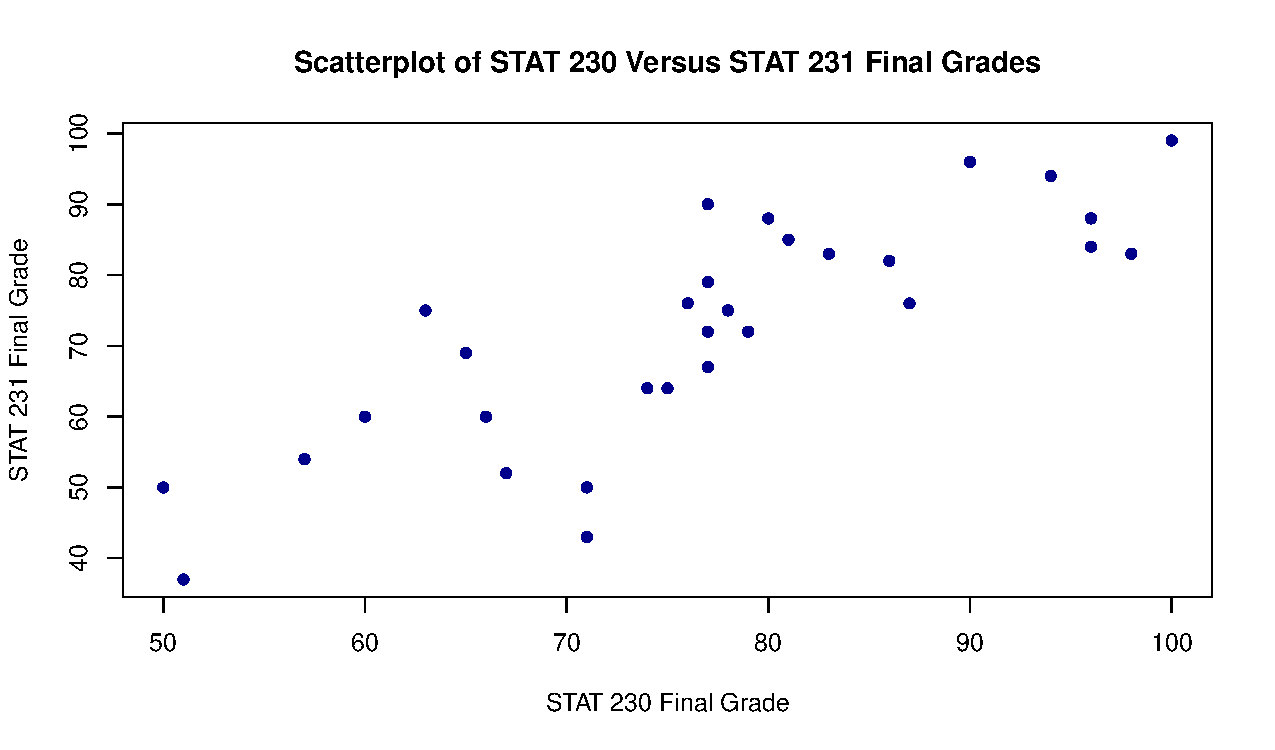
\includegraphics[width=\maxwidth]{figure/unnamed-chunk-3-1} 
\end{knitrout}
    %\end{noindent}
\end{Example}
\subsection{Least Squares Estimates}
%\begin{noindent}
\begin{knitrout}
\definecolor{shadecolor}{rgb}{0.969, 0.969, 0.969}\color{fgcolor}
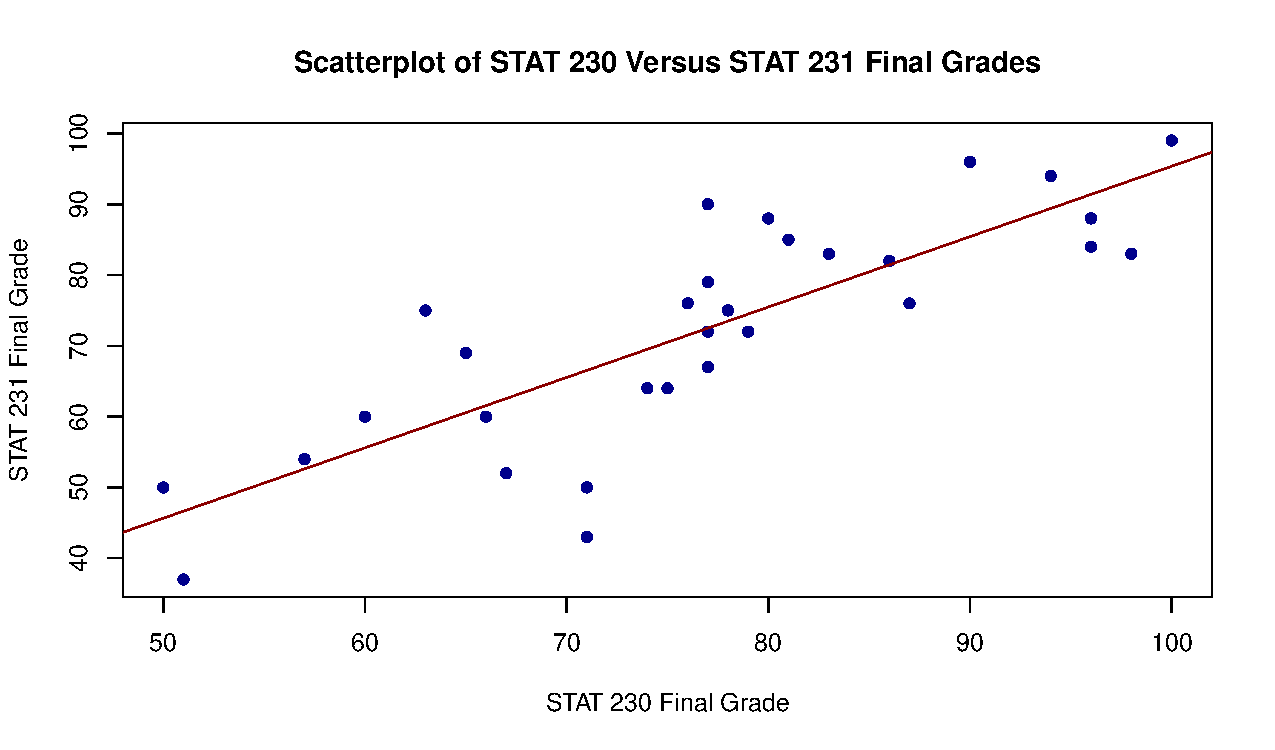
\includegraphics[width=\maxwidth]{figure/unnamed-chunk-4-1} 
\end{knitrout}
%\end{noindent}
To determine the fitted line $ y=\alpha+\beta x $, which minimizes the sum of the squares
of the distances between the observed points and the fitted line.

We need to find the values of $ \alpha $ and $ \beta $ which minimize
\[g(\alpha, \beta)=\sum_{i=1}^{n}(y_{i}-\alpha-\beta x_{i})^{2}.\]
These values are determined by simultaneously solving the equations
\begin{align*}
    \frac{\partial g}{\partial \alpha} & =\frac{\partial}{\partial \alpha} \sum_{i=1}^{n}(y_{i}-\alpha-\beta x_{i})^{2}=\sum_{i=1}^{n} 2(y_{i}-\alpha-\beta x_{i})(-1)=0,    \\
    \frac{\partial g}{\partial \beta}  & =\frac{\partial}{\partial \beta} \sum_{i=1}^{n}(y_{i}-\alpha-\beta x_{i})^{2}=\sum_{i=1}^{n} 2(y_{i}-\alpha-\beta x_{i})(-x_{i})=0.
\end{align*}
These equations can be written as
\begin{equation}\tag*{(1)}\label{6.1eq1}
    \bar{y}-\alpha-\beta \bar{x}=0,
\end{equation}
\begin{equation}\tag*{(2)}\label{6.1eq2}
    \sum_{i=1}^{n}(y_{i}-\alpha-\beta x_{i})(x_{i})=0.
\end{equation}
From equation~\ref{6.1eq1}, we obtain $ \alpha=\bar{y}-\beta \bar{x} $ which
we can substitute into equation~\ref{6.1eq2} to obtain
\[\sum_{i=1}^{n} x_{i}\bigl[y_{i}-\bar{y}-\beta(x_{i}-\bar{x})\bigr]=0,\]
or
\[\beta=
    \frac{\sum\limits_{i=1}^{n} x_{i}(y_{i}-\bar{y})}
    {\sum\limits_{i=1}^{n} x_{i}(x_{i}-\bar{x})}
    =\frac{\sum\limits_{i=1}^{n}(x_{i}-\bar{x}) y_{i}}
    {\sum\limits_{i=1}^{n}(x_{i}-\bar{x})^{2}}
    =\frac{\sum\limits_{i=1}^{n}(x_{i}-\bar{x})(y_{i}-\bar{y})}
    {\sum\limits_{i=1}^{n}(x_{i}-\bar{x})^{2}}
    =\frac{S_{x y}}{S_{x x}}.\]
Therefore, the least squares estimates are
\[\alpha=\hat{\alpha}=\bar{y}-\hat{\beta} \bar{x},
    \qquad \beta=\hat{\beta}=\frac{S_{x y}}{S_{x x}}.\]
And, the equation of the fitted line is
\[y=\hat{\alpha}+\hat{\beta} x.\]
\subsection{STAT 231 Versus STAT 230 Final Grades}
For the STAT 230/231 data, we have the following
\[\bar{x}=\frac{2302}{30}=76.7333,\qquad\bar{y}=\frac{2167}{30}=72.2333.\]
\[S_{x x}=5135.8667,\qquad S_{x y}=5106.8667,\qquad S_{y y}=7585.3667.\]
\[\hat{\beta}=\frac{S_{x y}}{S_{x x}}=\frac{5106.8667}{5135.8667}=0.9944.\]
\[\hat{\alpha}=\bar{y}-\hat{\beta} \bar{x}=72.2333-(0.9944)(76.7333)=-4.0667.\]
The fitted line is
\[y=-4.0667+0.9944 x.\]
\end{document}
